\section{Development and Implementation}
\label{development}

Our development efforts are divided into sections based on our data flow architecture.  There is some overlap of effort in the data preprocessing step as this is the area of our development where Simulation and Machine Learning meet.  We describe each development stage in detail in the following subsections.

\subsection{Simulation}
The machine learning algorithm we implemented requires training for it to accurately predict an atom location when given just the CCD image. Thus, we first need to generate a large training set consisting of pairs of atom locations with CCD images. This is done by simulating CCD images for the atom located at different points.

The essence of the simulation is starts with a flourescent atom at a chosen location, and then simulating how light emitted from the atom is refracted by the lens system and appears on the CCD screen. We opted for a classical raytracing approach. Rays are emitted in a random direction from the atom, and obey refraction via Snell's Law as they pass interfaces between different materials. When the rays intersect with the CCD plane, we increment an array value corresponding to which CCD pixel it hit.

\subsubsection{Raytracer Development}
A custom barebones raytracer was designed from the ground up in C, the key design goals being that it should be simplistic, fast, and readily parallelizable. This was done since the features of most raytracing systems are unnessesary for our application, in part because:
\begin{itemize}
\item We only need first order refracted rays. No higher order or reflected rays are needed.
\item We apriori know the order in which the rays will intersect surfaces.
\item Elements of graphical raytracing systems are more extravagant than the simple intensity plots we need.
\end{itemize}

Some important features that were implemented in the raytracer:
\begin{itemize}
\item Standard vector operations (projections, cross products, ray extrapolations, etc.)
\item Structure for defining arbitrary surfaces and refractive indicies.
\item Ray/Surface intersection routine.
\item Calculation of surface normals.
\item Implementation of Snell's law.
\item Ray refraction routine.
\item CCD image screen with histogram binning.
\end{itemize}
Each of these features were tested independantally by plotting ray traces with gnuplot. This was done in preparation for the more complex system with custom optics, which is harder to verify.

\subsubsection{Imaging System}
An imaging system consisting of a pair of custom aspheric lenses was then implemented with our raytracer surfaces. The system consists of five surfaces in all. The first two surfaces form the initial aspheric lens, the second two surfaces form the second aspheric lens, and the final surface forms the CCD image plane.

\begin{figure}
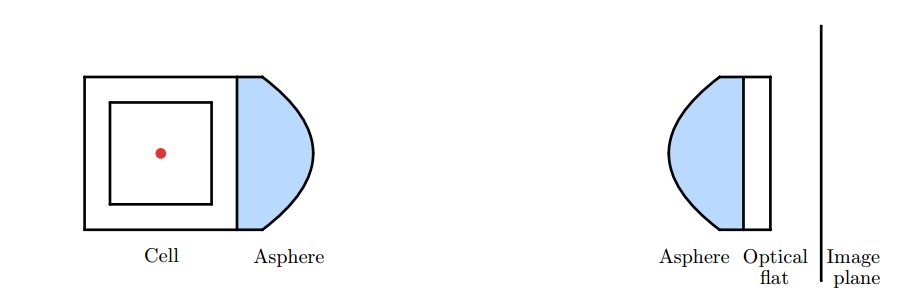
\includegraphics[scale=0.5]{asphere.png}
\caption{Scale model of the atom imaging system.}
\end{figure}

For completeness, the spacing between the lenses is $90$mm, the focal point is $5mm$ from the lens, and lastly, the asphere lens profiles are given by
\begin{equation}
  Z(r) = \frac{ C r^2}{1 + \sqrt{1-(1+k)C^2r^2}} + \sum_{i=0}^{10}D_{2i}r^{2i}
\end{equation}
with the constants
\begin{equation}
\begin{array}{|c|c|}
\hline
\text{Parameter} & \text{Value} \\
\hline
C & -0.128 \\
k & -0.824 \\ 
D_0 & 17.705 \\
D_2 & 2.11*10^{-2} \\
D_4 & 8.71*10^{-2} \\
\hline
\end{array}
\end{equation}



\subsection{Data Preprocessing}

%Ran talks about filtering here...
The original picture is designed to be 100 times 100 pixels matrix in each slice. The data preprocessing build a noise maker and filtering mechanism before the slices of matrix are actually applied to the classifier. It actually simulates a half transparent mask before the camera practically. The image generated by such mask adds Poisson distributed random number to every pixels of the image. A Poisson distribution stands for discrete probability that can give a number of events occurring in a fixed interval of time or space if events are independent with the average of $\lambda$. The value of $\lambda$ is switched between different proposed number in real test. Filtering, on the other hand, is clearing the influence caused by the noises. The filtering mechanism generally follows the work in course lab 8. A Gaussian distribution based figure blur decreases the degree of distribution caused by Poisson distribution based noises. Then, the Prewitt gradient filters all unnecessary noise with only structure, which contains the lines of rays, left.

The feature scaling step is handled in the logistic regression classifier as it is a simple extension to data loading after the instance have been loaded into memory.  We use efficient a C++ template library for linear algebra \cite{Eigen} that provides efficient matrix operations that can quickly perform the broadcasting operations necessary for feature scaling.  In addition, the distributed implementation of our algorithm lends itself well to efficient data partitioning, which ensures that this preprocessing step will scale.  However, feature scaling in a distributed setting is slightly more complex in that it requires knowledge of the global min and max for the entire dataset across all nodes.  The min/max vectors is quickly computed using an Allreduce step with MPI's MIN/MAX reduction operators. Each node then formats its section of the data using a single call feature scaling utility function.

\subsection{Machine Learning}
We have developed a distributed logistic regression classifier using MPI to train on massive amounts of data efficient.  The classifier is capable of multi-class classification and mini-batch processing.  During training, nodes communicate with each other to both build the model and perform parameter updates.

The model building step includes data loading, feature scaling, and label formating. During data loading, each node loads a portion of the instances the provided data directory based on its task ID and the total number of tasks in the communication world.  It is important to note that the instance file names are first loaded into a vector and then randomized to ensure that mini-batch processing have a consistent sample of the data with each iteration.  After the data is loaded, feature scaling is performed as described above.  The label formating step uses a custom MPI operator in an Allreduce call to generate global unique label set.  The unique label set is used at each node to generate a label matrix from the label vector for 1-vs-all classification.

The model training involves iterative updates to a set of global parameters.  During each update, the nodes compute a portion gradient update using a subset of the data they are responsible for based on the batch size.  The collective gradient update is computed using an Allreduce call to sum each contribution followed by a normalization step on each node based on the total number of instances contributing to the update.  The new parameter set (identical on all nodes) is then tested for convergence and used for the next iteration.

Training is finished when either the gradient has converged or the maximum number of iterations has been reached.  The Master node saves the trained model parameters to the a file to be loaded on a single node for testing.  The testing program generates a set of class membership probabilities for each instance in the given data directory.  The chosen class is simply the maximum probability found in the probabilities set for each instance.  We also use the probabilities to generate the visualizations of the models \emph{beliefs} about an atoms location for each instance.

\subsection{Visualization}
Visualization is particularly important for visualizing three dimensional volumes, and it may become essential for feedback as to whether our simulations are functioning properly, and for our presenting our project results. However, our project focus is not on programming the visualization methods ourselves, but using existing tools such as Visit or ParaView.

The main items to be visualized are the rays traced through the imaging system, the CCD images, and finally a prediction of the atom location given a CCD image. We can also use these tools for post processing on the image data to highlight features for the benefit of the machine learning algorithm.